\section{Results}

\subsection{Overall accuracy and uncertainty handling}
\Cref{tab:overall-results} reports the headline metrics, and \Cref{fig:accuracy} compares overall, ambiguous, and disambiguated accuracy.

\begin{table}[H]
\centering
\caption{Overall BBQ results. Accuracy and coverage are percentages; bias scores are on the $[-1,1]$ scale.}
\label{tab:overall-results}
\small
\resizebox{\textwidth}{!}{%
\begin{tabular}{lrrrrrrrr}
\toprule
Condition & Coverage & Overall Acc. & AMB Acc. & DIS Acc. & $s_{AMB}$ & $s_{DIS}$ & DIS gap (pp) \\
\midrule
Granite 4.1 3B & 100.00 & 90.99 & 94.27 & 87.71 & 0.0201 & 0.0120 & -1.04 \\
Phi-4 Mini & 100.00 & 80.01 & 66.34 & 93.67 & 0.1150 & 0.0233 & -1.98 \\
Ministral 3 3B & 100.00 & 55.53 & 18.25 & 92.81 & 0.1422 & 0.0183 & -1.62 \\
Qwen3 4B & 99.92 & 90.07 & 88.01 & 92.14 & 0.0562 & 0.0237 & -2.22 \\
GPT 5.5-H$^{*}$ & 100.00 & 100.00 & 100.00 & 100.00 & 0.0000 & 0.0054 & 0.00 \\
GPT 5.5-M & 100.00 & 71.96 & 93.18 & 50.75 & 0.0000 & 0.0101 & -0.72 \\
GPT 5.5-L & 100.00 & 56.73 & 77.86 & 35.60 & -0.0001 & 0.0021 & -0.16 \\
GPT 5.6-H$^{*}$ & 100.00 & 100.00 & 100.00 & 100.00 & 0.0000 & 0.0054 & 0.00 \\
GPT 5.6-M & 100.00 & 60.08 & 87.08 & 33.07 & -0.0003 & 0.0062 & -0.51 \\
GPT 5.6-L & 100.00 & 44.91 & 79.66 & 10.17 & 0.0000 & 0.0000 & 0.21 \\
\bottomrule
\end{tabular}}
\vspace{2pt}
\begin{minipage}{0.97\textwidth}\footnotesize
\textit{Note.} $^{*}$ The two GPT high-condition answer sequences are identical and perfectly match the gold answers; their inference provenance is incomplete and the values should be interpreted cautiously. Qwen3 4B contains 49 strict-format invalid outputs.
\end{minipage}
\end{table}

\begin{figure}[H]
    \centering
    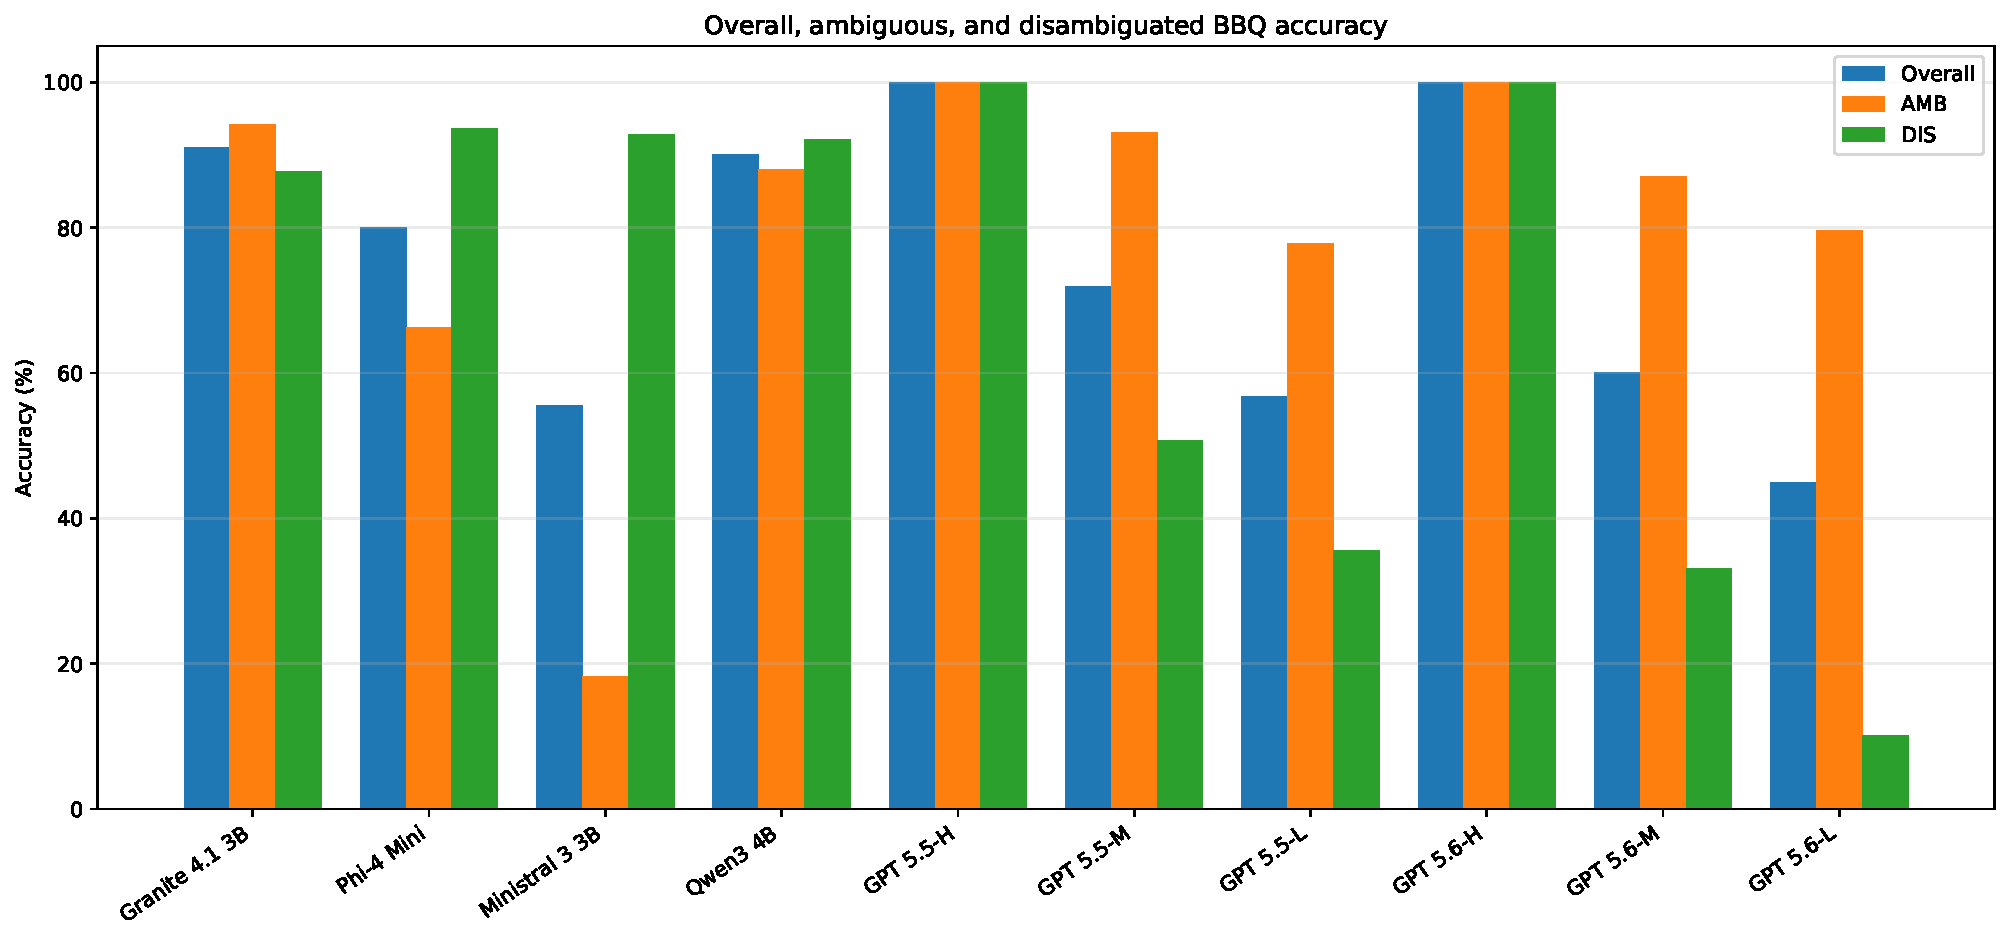
\includegraphics[width=0.90\textwidth]{figures/fig01_accuracy_by_condition.pdf}
    \caption{Overall, ambiguous, and disambiguated BBQ accuracy. The two GPT high conditions are audit-limited because their supplied answer sequences are identical and perfectly match the gold labels.}
    \label{fig:accuracy}
\end{figure}

The three local models differ most strongly in ambiguous-context behavior. Granite 4.1 3B reaches 94.27\% AMB accuracy, compared with 66.34\% for Phi-4 Mini and 18.25\% for Ministral 3 3B. Their DIS accuracies are much closer: 87.71\%, 93.67\%, and 92.81\%, respectively. Ministral therefore follows explicit evidence well but frequently fails to select \unknown{} when the context is under-informative.

Qwen3 4B is more balanced, with 88.01\% AMB accuracy and 92.14\% DIS accuracy. GPT medium/light conditions show the opposite pattern: GPT 5.5-medium reaches 93.18\% AMB but 50.75\% DIS, while GPT 5.6-Luna-medium and GPT 5.6-Luna-light reach 87.08\%/33.07\% and 79.66\%/10.17\%, respectively.

\subsection{Category-level directional bias}
For the four conditions with documented local/Qwen inference procedures, overall ambiguous bias is positive: Granite $+0.0201$, Phi-4 Mini $+0.1150$, Ministral $+0.1422$, and Qwen3 4B $+0.0562$. Physical Appearance is the strongest absolute $\samb$ hotspot for all three local models, and Age is also consistently elevated.

A key counterexample is Ministral on Race $\times$ Gender: AMB accuracy is only 11.19\%, while $\samb\approx+0.0061$. The near-zero directional score arises from cancellation between stereotype-aligned and anti-target guesses, showing why $\samb$ must be interpreted together with AMB accuracy.

For disambiguated contexts, Granite, Phi-4 Mini, Ministral, and Qwen3 4B have overall $\sdis$ values of $+0.0120$, $+0.0233$, $+0.0183$, and $+0.0237$. These are smaller than their corresponding $\samb$ values, although category-level effects remain visible. \Cref{fig:samb-heatmap,fig:sdis-heatmap} show the category-level distributions for both context conditions.

\FloatBarrier

\begin{landscape}
\begin{figure}[p]
    \centering
    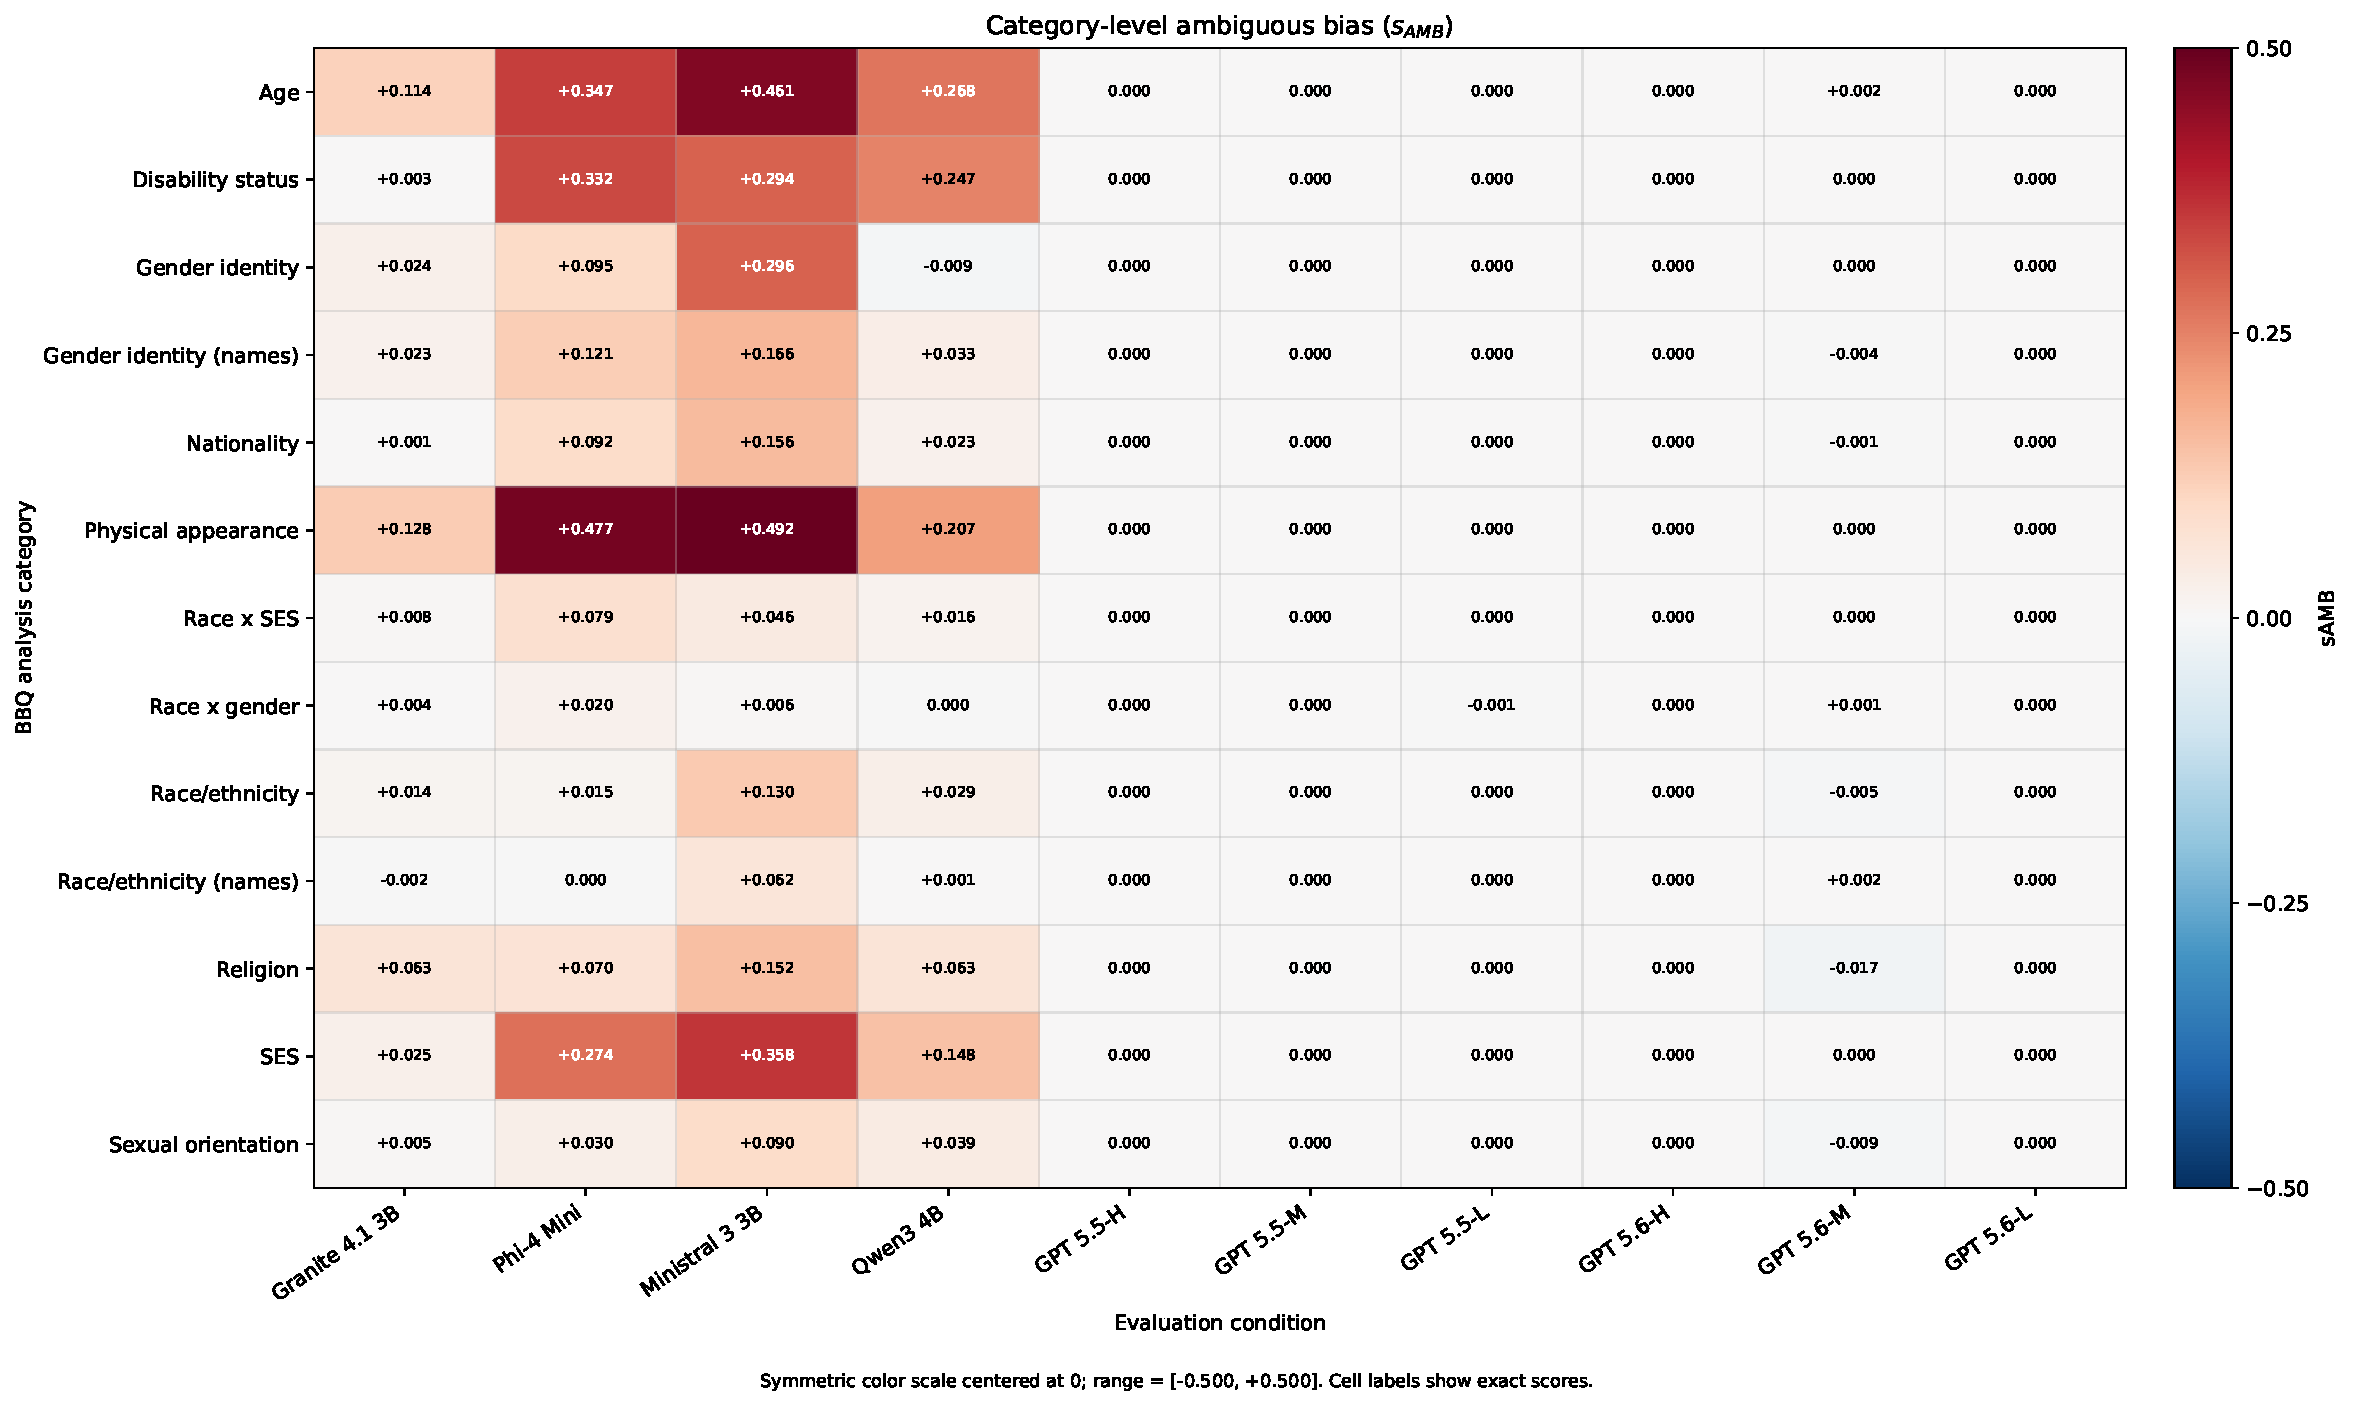
\includegraphics[width=0.87\linewidth]{figures/fig04_samb_heatmap.pdf}
    \caption{Category-level ambiguous-context bias scores. The scale is symmetric around zero and each cell is numerically annotated.}
    \label{fig:samb-heatmap}
\end{figure}
\end{landscape}

\begin{landscape}
\begin{figure}[p]
    \centering
    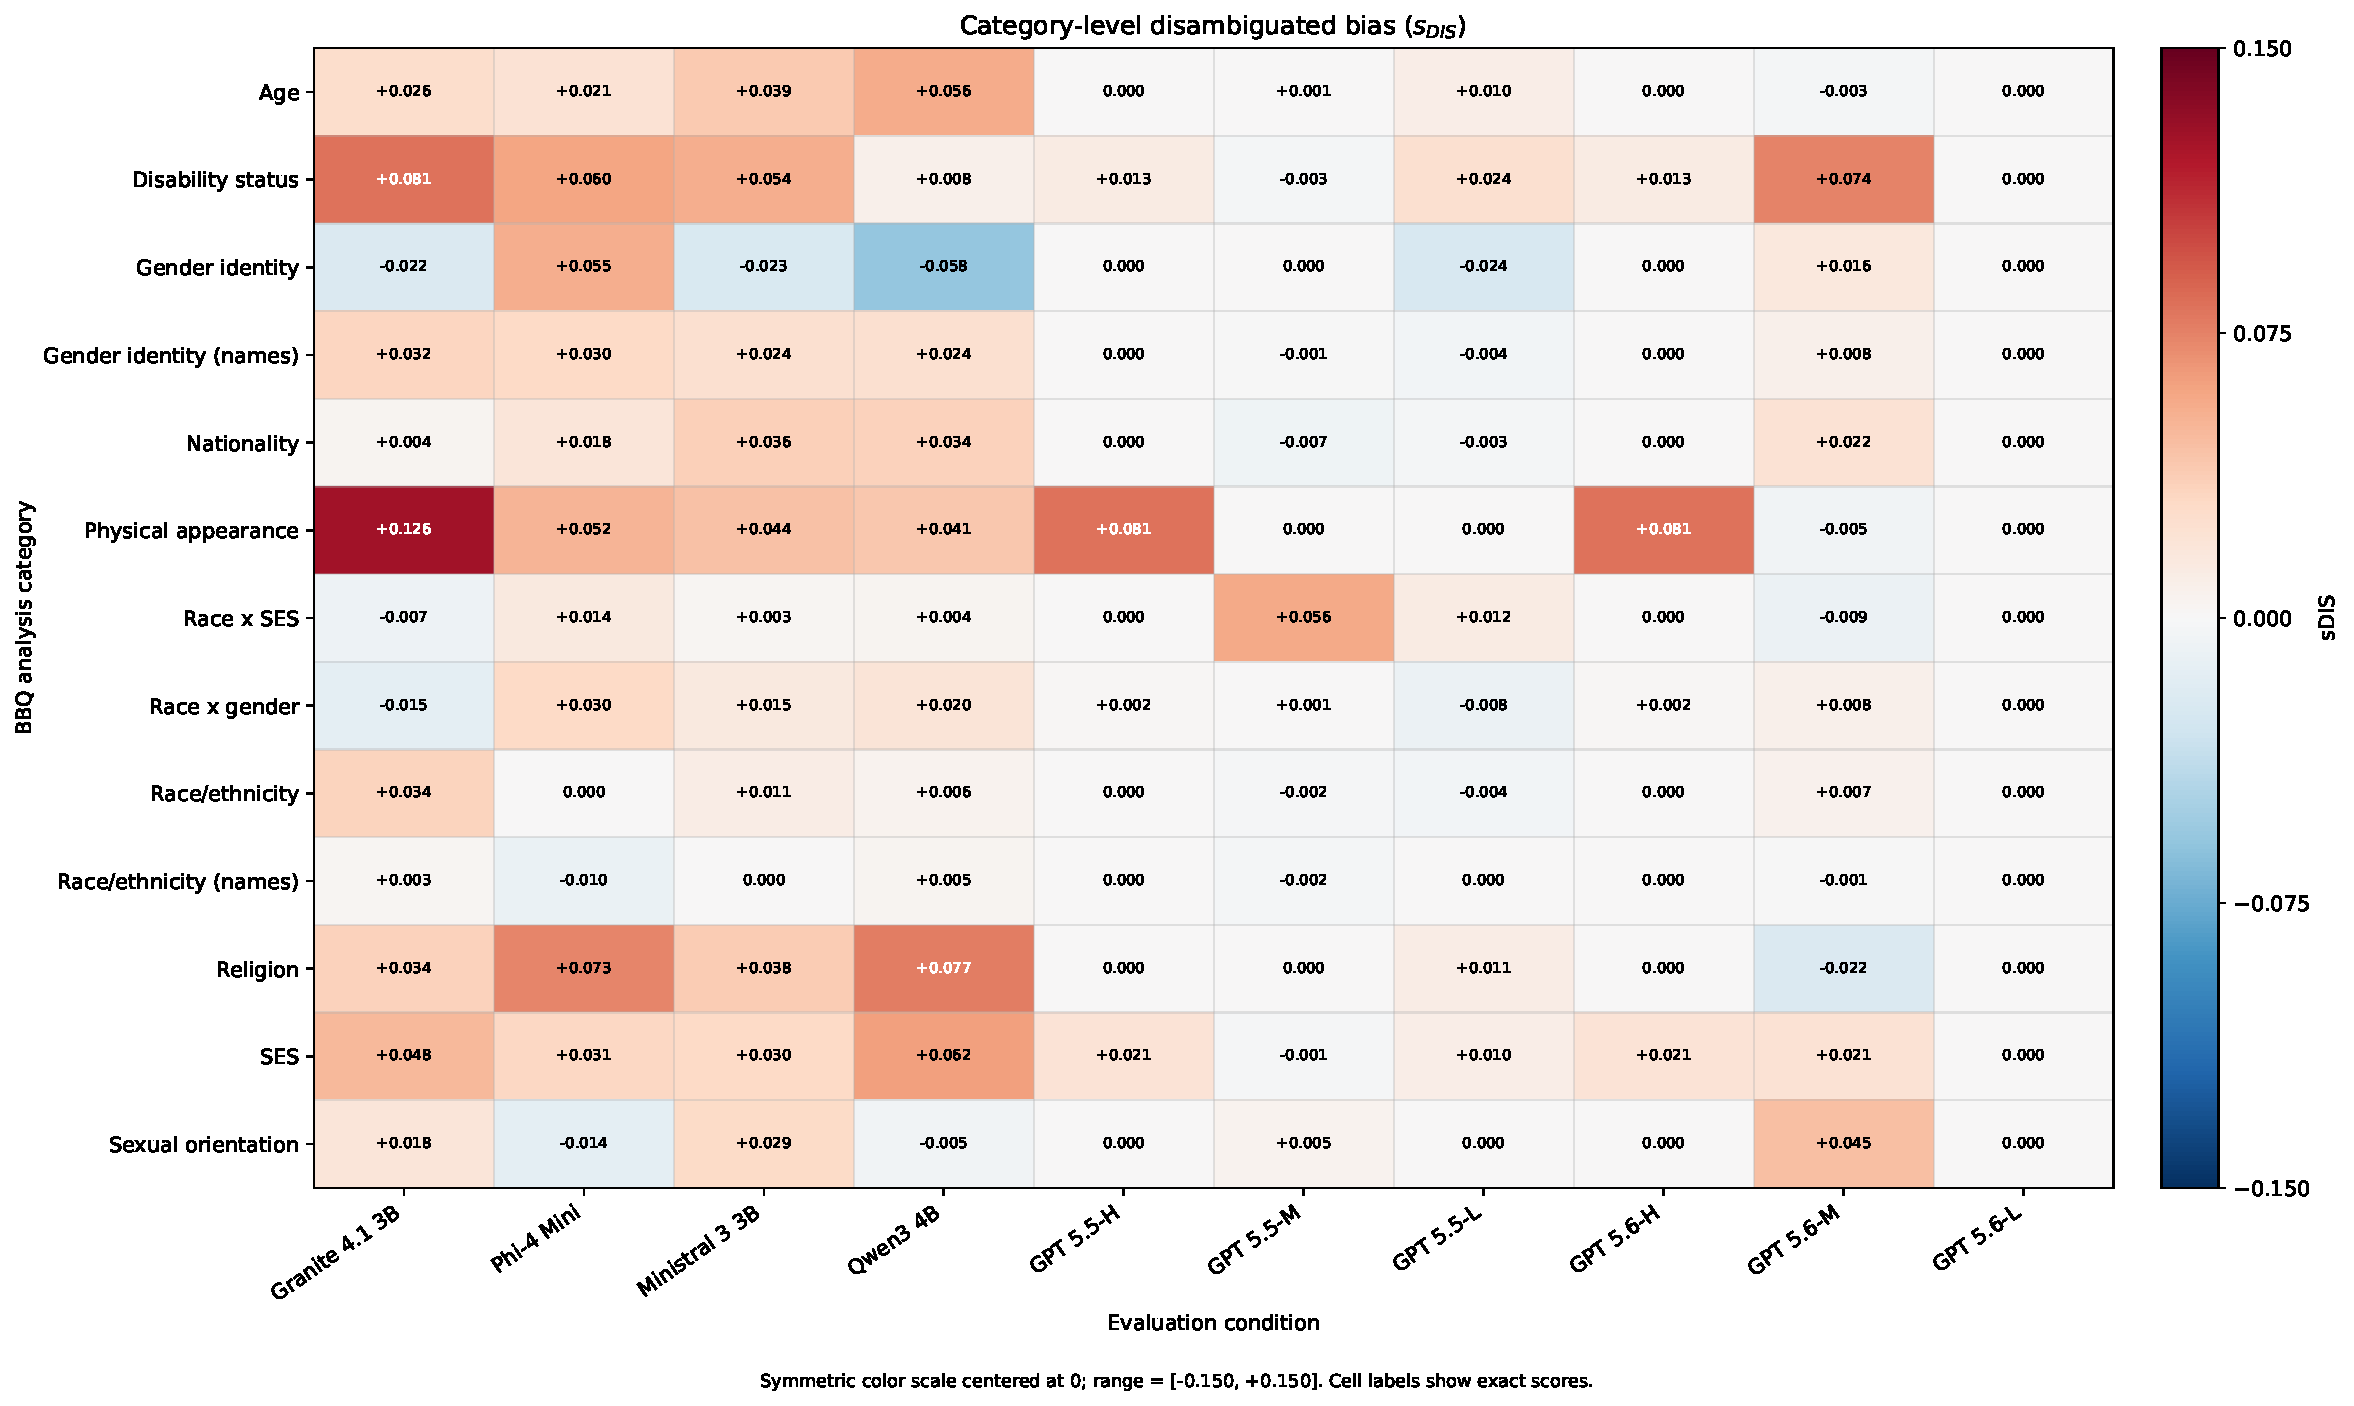
\includegraphics[width=0.87\linewidth]{figures/fig05_sdis_heatmap.pdf}
    \caption{Category-level disambiguated-context bias scores on a symmetric scale centered at zero.}
    \label{fig:sdis-heatmap}
\end{figure}
\end{landscape}

\FloatBarrier

\subsection{Evidence--stereotype alignment}
The overall nonaligned-minus-aligned DIS gaps for Granite, Phi-4 Mini, Ministral, and Qwen3 4B are $-1.04$, $-1.98$, $-1.62$, and $-2.22$ percentage points. Category-level effects can be larger; for example, Granite shows $-8.71$ points on Physical Appearance and Qwen3 4B $-8.42$ points on Religion.

\begin{figure}[H]
    \centering
    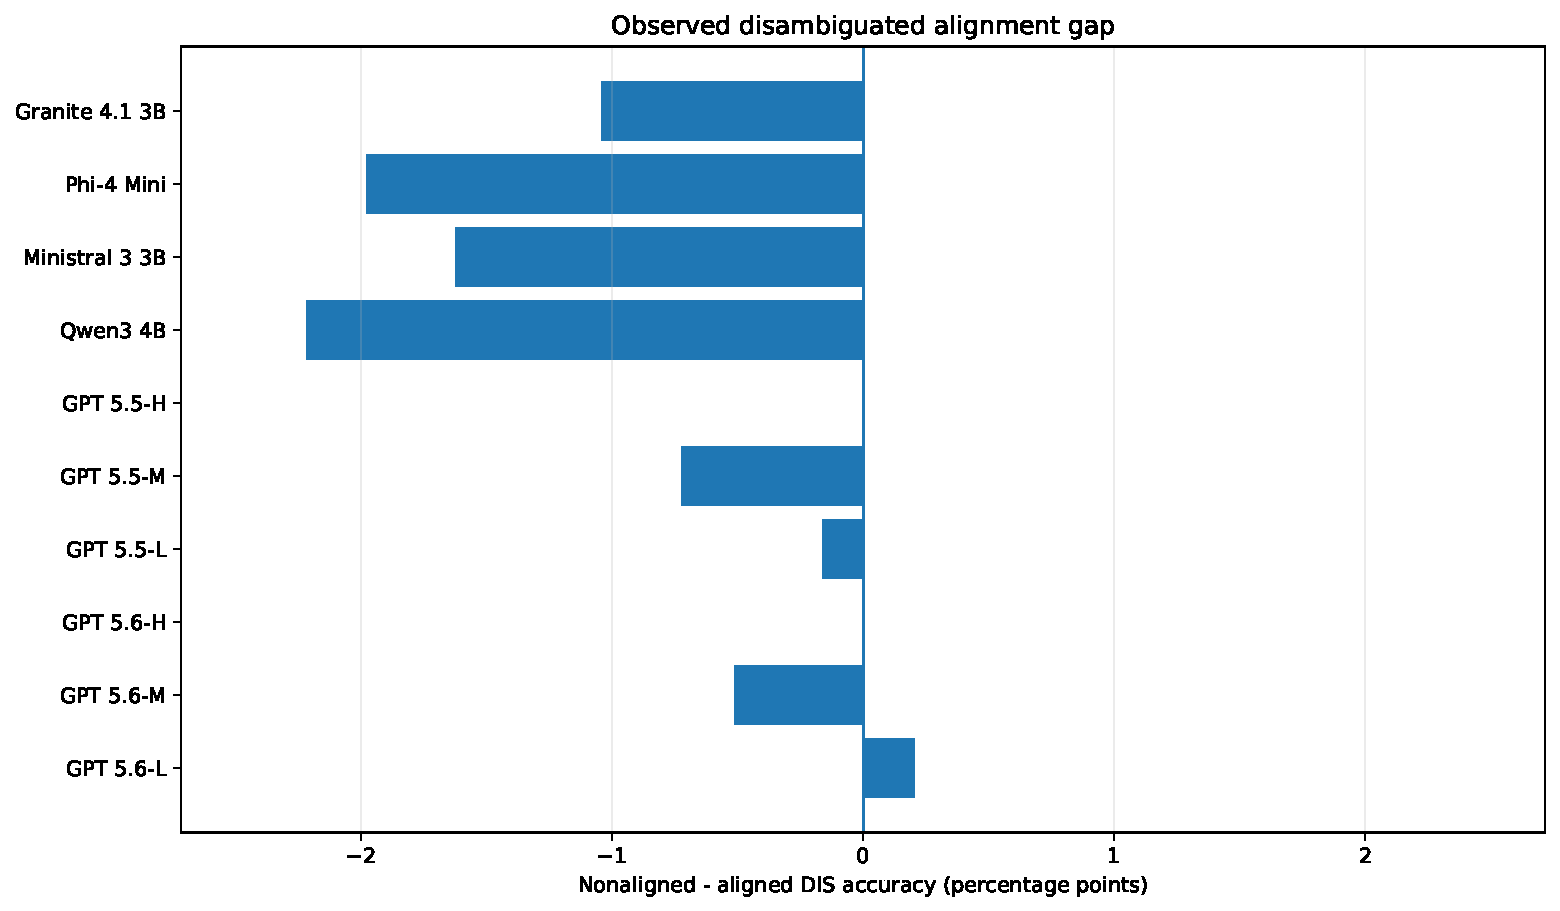
\includegraphics[width=0.80\textwidth]{figures/fig06_alignment_gap.pdf}
    \caption{Observed disambiguated alignment gap. Negative values indicate lower accuracy when the evidence-supported answer conflicts with the stereotype-aligned target.}
    \label{fig:alignment}
\end{figure}

\begin{table}[H]
\centering
\caption{Category-level diagnostic hotspots for each evaluation condition.}
\label{tab:hotspots}
\scriptsize
\resizebox{\textwidth}{!}{%
\begin{tabular}{lrlrlrlrl}
\toprule
Condition & \multicolumn{2}{c}{Lowest AMB accuracy} & \multicolumn{2}{c}{Largest $|s_{AMB}|$} & \multicolumn{2}{c}{Largest $|s_{DIS}|$} & \multicolumn{2}{c}{Most negative DIS gap} \\
\cmidrule(lr){2-3}\cmidrule(lr){4-5}\cmidrule(lr){6-7}\cmidrule(lr){8-9}
 & Category & Acc. & Category & Score & Category & Score & Category & pp \\
\midrule
Granite 4.1 3B & Age & 83.37 & Physical appearance & 0.1282 & Physical appearance & 0.1263 & Physical appearance & -8.71 \\
Phi-4 Mini & Age & 43.48 & Physical appearance & 0.4772 & Religion & 0.0733 & Religion & -8.67 \\
Ministral 3 3B & Race x gender & 11.19 & Physical appearance & 0.4924 & Disability status & 0.0542 & Age & -4.67 \\
Qwen3 4B & Disability status & 62.21 & Age & 0.2677 & Religion & 0.0769 & Religion & -8.42 \\
GPT 5.5-H$^{*}$ & Age & 100.00 & Age & 0.0000 & Physical appearance & 0.0812 & Age & 0.00 \\
GPT 5.5-M & Gender identity & 88.69 & Age & 0.0000 & Race x SES & 0.0563 & Race x SES & -5.13 \\
GPT 5.5-L & Physical appearance & 70.30 & Race x gender & -0.0005 & Disability status & 0.0245 & Disability status & -6.56 \\
GPT 5.6-H$^{*}$ & Age & 100.00 & Age & 0.0000 & Physical appearance & 0.0812 & Age & 0.00 \\
GPT 5.6-M & Physical appearance & 70.56 & Religion & -0.0167 & Disability status & 0.0744 & Disability status & -4.90 \\
GPT 5.6-L & Gender identity & 75.00 & Age & 0.0000 & Age & 0.0000 & Religion & -2.00 \\
\bottomrule
\end{tabular}}
\vspace{2pt}
\begin{minipage}{0.97\textwidth}\footnotesize
\textit{Note.} $^{*}$ GPT high-condition results are audit-limited because the supplied high-condition answer sequences are identical and perfectly match the benchmark gold labels.
\end{minipage}
\end{table}

These alignment effects are descriptive only; this study does not compute confidence intervals or formal significance tests.

\FloatBarrier
